

%\tikzset{every picture/.style={line width=0.75pt}} %set default line width to 0.75pt        

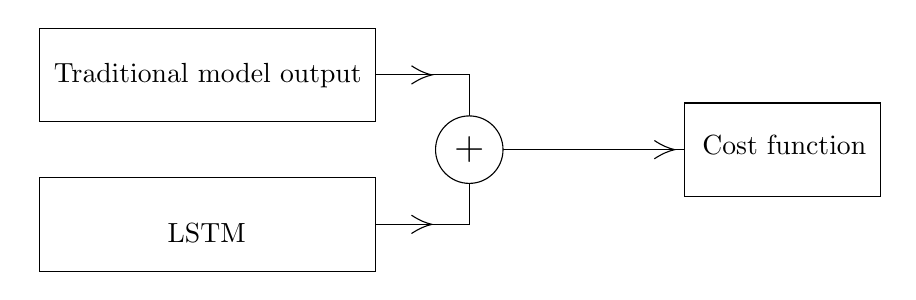
\begin{tikzpicture}[x=0.75pt,y=0.75pt,yscale=-0.9,xscale=0.9]
%uncomment if require: \path (0,300); %set diagram left start at 0, and has height of 300

%Shape: Right Angle [id:dp6736520719365272] 
\draw   (320,50) -- (370,50) -- (370,90) ;
%Shape: Right Angle [id:dp1824696211077277] 
\draw   (370,90) -- (370,130) -- (320,130) ;
%Straight Lines [id:da5169071611896188] 
\draw    (370,90) -- (485,90) ;
\draw [shift={(480,90)}, rotate = 180] [color={rgb, 255:red, 0; green, 0; blue, 0 }  ]   (10.93,-4.9) .. controls (6.95,-2.3) and (3.31,-0.67) .. (0,0) .. controls (3.31,0.67) and (6.95,2.3) .. (10.93,4.9)   ;
\draw [shift={(350,50)}, rotate = 180] [color={rgb, 255:red, 0; green, 0; blue, 0 }  ]   (10.93,-4.9) .. controls (6.95,-2.3) and (3.31,-0.67) .. (0,0) .. controls (3.31,0.67) and (6.95,2.3) .. (10.93,4.9)   ;
\draw [shift={(350,130)}, rotate = 180] [color={rgb, 255:red, 0; green, 0; blue, 0 }  ]   (10.93,-4.9) .. controls (6.95,-2.3) and (3.31,-0.67) .. (0,0) .. controls (3.31,0.67) and (6.95,2.3) .. (10.93,4.9)   ;
%\draw   (336,44.92) .. controls (340.03,47.37) and (344.07,48.84) .. (348.1,49.33) .. controls (344.07,49.82) and (340.03,51.3) .. (336,53.75) ;
%\draw   (338.5,130.08) .. controls (342.53,132.54) and (346.57,134.01) .. (350.6,134.5) .. controls (346.57,134.99) and (342.53,136.46) .. (338.5,138.92) ;

% Text Node
\draw    (140,25) -- (320,25) -- (320,75) -- (140,75) -- cycle  ;
\draw (230,50.2) node   [align=left] {\begin{minipage}[lt]{122.67200000000003pt}\setlength\topsep{0pt}
\begin{center}
Traditional model output
\end{center}

\end{minipage}};
% Text Node
\draw    (140,105) -- (320,105) -- (320,155) -- (140,155) -- cycle  ;
\draw (229.4,134.6) node   [align=left] {\begin{minipage}[lt]{122.67200000000003pt}\setlength\topsep{0pt}
\begin{center}
LSTM
\end{center}

\end{minipage}};
% Text Node
\draw  [fill={rgb, 255:red, 255; green, 255; blue, 255 }  ,fill opacity=1 ]  (370, 90) circle [x radius= 18.06, y radius= 18.06]   ;
\draw (370,90) node   [align=left] {\begin{minipage}[lt]{16.864pt}\setlength\topsep{0pt}
\begin{center}
{\Large +}
\end{center}

\end{minipage}};
% Text Node
\draw    (485,65) -- (590,65) -- (590,115) -- (485,115) -- cycle  ;
\draw (538.6,87.4) node   [align=left] {\begin{minipage}[lt]{68pt}\setlength\topsep{0pt}
\begin{center}
Cost function
\end{center}

\end{minipage}};


\end{tikzpicture}

